\documentclass{article}

\usepackage{float,algorithm,graphicx,amsmath,amsfonts,verbatim}
\usepackage[hyphens]{url}
\usepackage[noend]{algpseudocode}

\title{Lab 9 - Convolutional Neural Networks}
\author{Kyle Swanson}
\date{January 24, 2018}

\setcounter{section}{-1}

\begin{document}

\maketitle

\section{Introduction}

In this lab we're going to be building neural networks to classify hand-written digits from the MNIST dataset. The input to our networks are going to be 28 x 28 pixel grayscale images, and the output will be a number between 0 and 9. MNIST images look like the following:

\begin{center}
    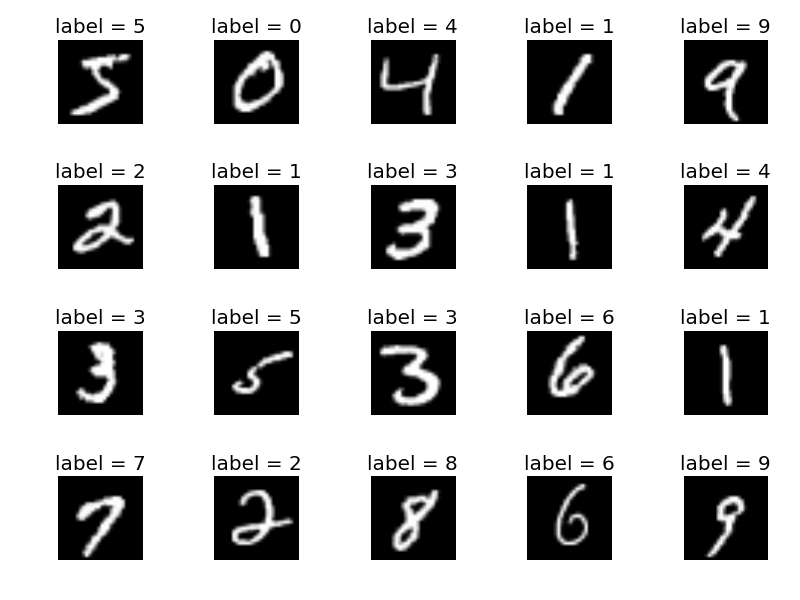
\includegraphics[width=0.75\textwidth]{mnist.png}
\end{center}

We will be building two different types of networks to classify these digits. First, we will be building a fully connected neural network (also called a multilayer perceptron), which is the basic neural network we talked about in Lectures 7 and 8 and built in Labs 7, 8, and 8.5. To use images as input, these networks flatten a 2D image into a 1D vector and pass the vector into the network, as seen below.

\begin{center}
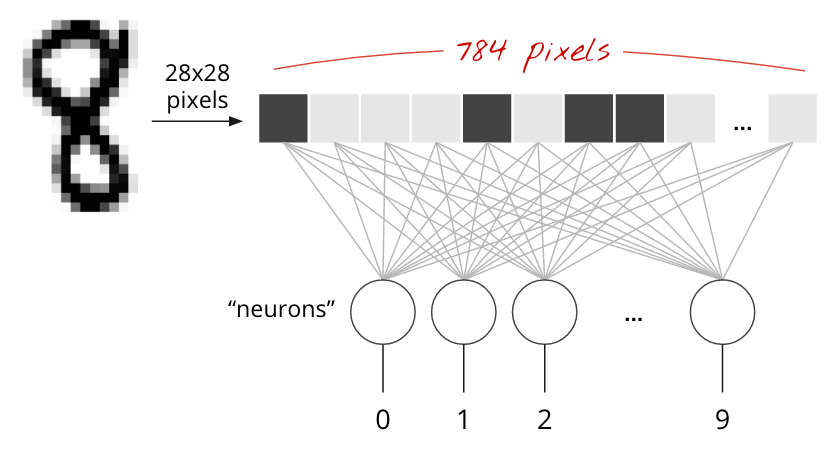
\includegraphics[width=0.75\textwidth]{mnist_fc.png}
\end{center}

After working with a fully connected network, we will try to classify digits using a convolutional neural network (CNN). CNNs are specifically designed to process images, and they work by passing filters over the image in its original form (no flattening) with each filter looking for specific features of the image (ex. straight lines for 1 and 7 or loops for 6 and 9). Below is a diagram illustrating a typical CNN.

\begin{center}
    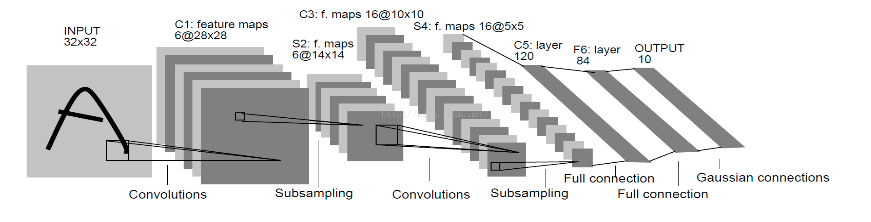
\includegraphics[width=\textwidth]{mnist_conv.png}
\end{center}

\section{Fully Connected Neural Network}

\subsection{Implementation}

Your first task is to build a fully connected neural network with two hidden layers using keras. Go into \texttt{lab9.py} and implement the function \texttt{build\_model\_fc}. This function should construct a keras Sequential model, and it should add the following layers:

\begin{itemize}
    \item Dense layer with 512 neurons and relu activation (hidden layer 1)
    \item Dropout layer with 0.2 dropout probability
    \item Dense layer with 512 neurons and relu activation (hidden layer 2)
    \item Dropout layer with 0.2 dropout probability
    \item Dense layer with \texttt{num\_classes} neurons and softmax activation (output layer)
\end{itemize}

Note that for the first layer, you need to specify that \texttt{input\_shape=input\_shape} so that keras knows how many weights to construct.

\subsection{Dropout}

The Dense layers are our usual hidden layers where each neuron in one layer is connected to each neuron in the next layer. The Dropout layers are not actual hidden layers but instead perform regularization on the Dense layers. They work by randomly ``dropping out" neurons in the hidden layers with a certain probability during training, meaning the activations of these neurons is set to 0 and they are essentially removed from the network (temporarily). This forces the remaining neurons to become more independent and robust because any neurons that they might normally rely on could be randomly dropped out. This helps the model generalize. Dropout is illustrated below.

\begin{center}
    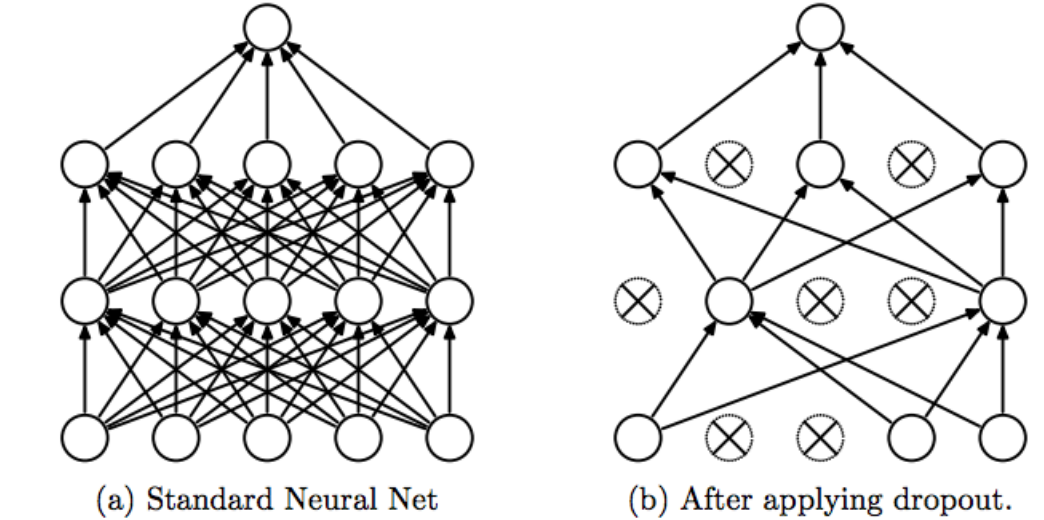
\includegraphics[width=\textwidth]{dropout.png}
\end{center}

For more information on dropout, take a look here: \url{https://medium.com/@amarbudhiraja/https-medium-com-amarbudhiraja-learning-less-to-learn-better-dropout-in-deep-machine-learning-74334da4bfc5}

\subsubsection{Running the code + activations}

Once your implementation is complete, go into \texttt{main.py}, uncomment Part 1, and run \texttt{python main.py}.

The first thing you'll see is an image of the \textit{activations} of the network. The activations of the network indicate which neurons respond most to the input image (i.e. which neurons have the largest output after applying the activation function). The image you see shows the activations for a specific MNIST image before the network has been trained, so these are activations based on random weights. The activations at the bottom of the image are the activations of the final layer, which is the layer outputting the probabilities of each class. You can see that almost all 10 output neurons are activated, indicating that the model doesn't know which number to guess.

After you close the image, the network will be trained for 10 epochs. Watch how the loss decreases and the accuracy increases. At the end you'll see the test loss and accuracy printed to the screen and you should see that this network performs very well ($\sim 98\%$ accuracy). Finally you'll see an image with the activations after training. This time only one neuron in the output layer (at the bottom of the image) is activated, indicating that this is the guess of the network. (Check that the guess of the network matches the actual digit in the image.) While the final layer activations are easy to interpret, it's hard to make sense of the activations of the hidden layers. For this reason, activations are more useful with convolutional neural networks where they more clearly show what parts of the image the network is looking at.

\section{Convolutional Neural Network}

\subsection{Implementation}

Now you will be building a convolutional neural network. Go into \texttt{lab9.py} and implement the function \texttt{build\_model\_conv}. This function should construct a keras Sequential model, and it should add the following layers:

\begin{itemize}
\item Conv2D layer with 32 3x3 filters and relu activation
\item Conv2D layer with 64 3x3 filters and relu activation
\item MaxPooling2D layer with pool size 2x2
\item Flatten layer
\item Dense layer with 128 neurons and relu activation
\item Dropout layer with 0.5 dropout probability
\item Dense layer with \texttt{num\_classes} neurons and softmax activation
\end{itemize}

\subsection{Running the code + activations}

When your implementation is complete, go into \texttt{main.py}, uncomment Part 2, and run \texttt{python main.py}.

As with the fully connected network, you'll first see the activations before training, then you'll see the loss and accuracy as the network trains (this time for only 2 epochs since this CNN is slower than the fully connnected network), and then you'll see the activations after training.

You should see that the convolutional network has slightly better accuracy than the fully connected network. While the difference is small for this dataset, convolutional networks significantly outperform fully connected networks on more difficult image tasks, and so convolutional neural networks are the standard neural network architecture to use when working with image data.

Note how the activations are much easier to interpret since CNNs work with the original square image and apply square filters rather than flattening the image into a single vector. Also compare the activations before training to those after training. Again note how the softmax activations at the bottom of the image are random before training but make a correct prediction after training. Look also at some of the activations in the convolutional layers and notice what the different filters are looking for (ex. horizontal lines or diagonal lines). Since digits are pretty simple there isn't too much to be learned from the activations, but for more complex tasks like object detection, activations can illustrate what the CNN is seeing.

If you're interesting in looking at activations on a set of real-world images, take a look here: \url{https://cs.stanford.edu/people/karpathy/convnetjs/demo/cifar10.html}

\end{document}
